\section{Architetture Software}
La \emph{\textcolor{cyan}{progettazione}} è la fase che segue la \emph{specifica} e
precede la \emph{codifica}. Descrive in che modo deve essere realizzato il progetto. Il suo
prodotto si chiama \emph{architettura}.

Esistono due tipi di \emph{progettazione}:
\begin{itemize}
    \item Progettazione di \textcolor{cyan}{alto livello}: lo scopo è identificare
        e scomporre il sistema in tanti piccoli sottosistemi e definire le loro inter-connessioni.
    \item Progettazione di \textcolor{cyan}{dettaglio}: si decide come ogni singolo \emph{sottosistema} deve
        essere realizzato.
\end{itemize}

Quindi l'\textcolor{cyan}{architettura} di un sistema software è la
struttura del sistema costituita dalle sue parti e dalle relazioni fra esse,
più le loro proprietà visibili all'esterno. Vengono considerati anche gli aspetti
\emph{\textcolor{cyan}{non funzionali}}.

Durante questa fase il sistema viene analizzato attraverso tre punti di vista:
\begin{itemize}
    \item Vista \textbf{\textcolor{cyan}{Comportamentale}} o \emph{component-and-connector}: questa vista descrive il sistema trattandolo
        come composizione di altri software. Quindi si specificano tutte le componenti (i software), che presentano delle \emph{interfacce},
        successivamente si descrivono le caratteristiche dei \emph{connettori} che collegano le varie componenti. Infine si
        analizza la struttura del sistema in esecuzione, infatti questa vista è molto utile per analizzare la qualità e le prestazioni del software e per documentare
        lo stile dell'architettura. 
    \item Vista \textbf{\textcolor{cyan}{Strutturale}}: permette di descrivere la struttura del sistema vedendolo
        come un insieme di \emph{classi} e/o \emph{packages}. È utile per analizzare le dipendenza tra le \emph{classi}/\emph{packages}
        e per progettare i test di \emph{unità} e di \emph{integrazione}.
    \item Vista \textbf{\textcolor{cyan}{Logica}} o di \emph{deployment}: descrive l'allocazione del software su più ambienti di esecuzione.
\end{itemize}

\subsection{Vista Comportamentale}

\begin{definition}[Componente]
    Una \textbf{\textcolor{cyan}{componente software}} è un'unità software indipendente
    e che può essere riusata da altri componenti. Incapsula un insieme di funzionalità e/o di
    dati di un sistema, restringendo l'accesso ad essi tramite la definizione di \emph{iterfacce}.
\end{definition}

\begin{figure}[H]
    \centering
    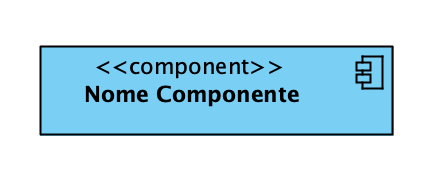
\includegraphics[scale=0.8]{img/component.png}
\end{figure}

\begin{definition}[Porti]
    I \textbf{\textcolor{cyan}{porti}} identificano i punti di interazione di un componente, ogni componente ne ha uno
    per ogni connessione che ha con altri componenti. Un \emph{porto} può richiedere una o più interfacce dello stesso tipo.
\end{definition}

\begin{figure}[H]
    \centering
    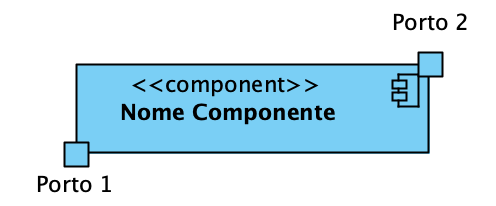
\includegraphics[scale=0.8]{img/porti.png}
\end{figure}

Le \emph{\textcolor{cyan}{interfacce}} possono essere rappresentate in modo esteso o in modo sintetico mediante l'uso
di \emph{forchette} (quando viene richiesta un'interfaccia) o \emph{lollipop} (quando l'interfaccia è fornita).

\begin{figure}[H]
    \centering
    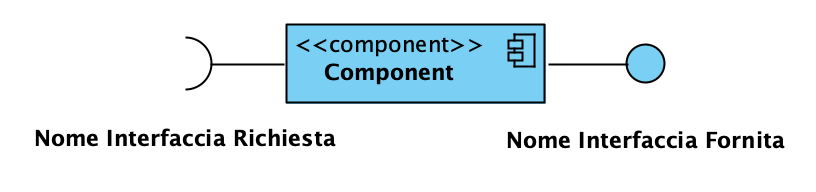
\includegraphics[scale=0.8]{img/lollipop.png}
    \caption{Modo Sintetico}
\end{figure}

\begin{figure}[H]
    \centering
    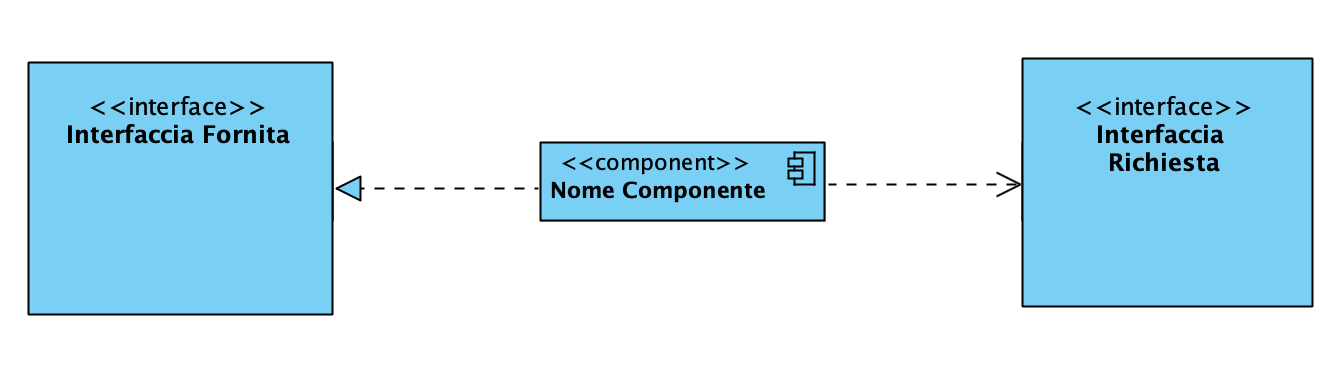
\includegraphics[scale=0.5]{img/interfacce.png}
    \caption{Modo Esteso}
\end{figure}

\begin{definition}[Connettori]
    I \textbf{\textcolor{cyan}{connettori}} sono i canali di comunicazione che collegano i \emph{porti} fra componenti
    diverse. Sul connettore è possibile indicare il \emph{protocollo di comunicazione} utilizzato fra \verb|<<...>>|.
\end{definition}

\subsubsection{Stili Architetturali}
\begin{definition}[Stile]
    Uno \textbf{\textcolor{cyan}{stile}} è una proprietà dell'architettura che ne caratterizza una famiglia con caratteristiche
    e interazioni fra componenti comuni.
\end{definition}

\paragraph{\textcolor{cyan}{Pipe \& Filter}}
Le componenti sono di tipo \emph{filtro}, ovvero effettuano delle trasformazioni sui dati
che provengono dai porti d'ingresso e li mandano sui porti d'uscita. I connettori, invece, sono di tipo
\emph{pipe}, ovvero un canale di comunicazione unidirezionale e che preserva l'ordine dei dati che entrano e che escono.

\paragraph{\textcolor{cyan}{Client-Server}}
Il sistema è formato da componenti che si comportano da \emph{client} e altri da \emph{server}.
Il client si connette a un server tramite un porto per richiedere un servizio, il server può ricevere connessioni da parte
di più client.

\paragraph{\textcolor{cyan}{Master-Slave}} È un caso particolare del
modello \emph{client-server}, in cui lo \emph{slave} (il server) può servire
un solo \emph{master} (client).

\paragraph{\textcolor{cyan}{Peer-to-Peer}} Tutti i componenti agiscono sia da client che da server, quindi nella
rappresentazione ci sarà un solo componente.

\paragraph{\textcolor{cyan}{Publish-Subscrive}} I componenti interagiscono tra loro
tramite l'annuncio di eventi, una componente può svolgere sia il ruolo di \emph{Publisher} (produttore di eventi) che di
\emph{Subscriber} (consumatore di eventi). Questo stile può coinvolgere anche un
intermediario chiamato \emph{broker}, che permette alle altre componenti di non interagire direttamente
fra loro e quindi di non essere consapevole delle indentià delle altre.

\paragraph{\textcolor{cyan}{Model-View-Controller}} Permette di isolare il \emph{\textcolor{cyan}{modello}},
ovvero le funzionalità e i dati del sistema, la \emph{\textcolor{cyan}{vista}}, quindi come viene rappresentato il modello, e il 
\emph{\textcolor{cyan}{controllore}}, che riceve l'input ed effettua le chiamate alle operazioni del modello.

\paragraph{\textcolor{cyan}{Coordinatore di Processi}} Prevede l'uso di un componente noto come
\emph{\textcolor{cyan}{coordinatore}}, che conosce la sequenza per realizzare il processo. Una volta ricevuta
la richiesta, chiama le componenti \emph{server} nell'ordine prefissato e successivamente fornisce una risposta.
I server non sono a conoscenza del loro ruolo, ma si limitano solo a fornire un servizio.

\subsection{Vista Strutturale}

Gli elementi di questa vista sono chiamati \emph{\textcolor{cyan}{moduli}}, ed essendo
classi o packages, le relazioni fra essi sono di ereditarietà, dipendenza o composizione.
Un \emph{package} può contenere un insieme di classi e/o di altri packages.

Questo tipo di vista è utile per fornire uno schema del codice e dei file sorgenti, non và utilizzato per le analisi dinamiche,
effettuate con viste \emph{comportamentali} e \emph{logistiche}.

Nelle classi, rispetto alla descrizione del \emph{dominio}, qui si specificano meglio
le loro operazioni.

\subsubsection{Vista Strutturale a Strati}

Gli elementi sono gli \emph{\textcolor{cyan}{strati}}, ovvero un insieme di moduli, che possono essere
raggruppati in \emph{segmenti}, inoltre implementano un'interfaccia pubblica, chiamata \emph{\textcolor{cyan}{macchina virtuale}} per i servizi che offrono.
La relazione fra gli strati è di tipo \verb|<<allowedToUse>>|, è antisimmetrica e non è transitiva.

\subsubsection{Vista Strutturale di Generalizzazione}

Gli elementi sono sempre i moduli, ma la relazione è solo di \emph{generalizzazione}.

\subsection{Vista Logistica}

In questa vista gli elementi possono essere \emph{hardware} (rappresentati da parallelepipedi) come l'ambiente di esecuzione, oppure
\emph{software} (con stereotipo \verb|<<artifact>>|), chiamati \emph{\textcolor{cyan}{artefatti}}, cioè qualsiasi file che viene utilizzato o prodotto
da un software da un sistema generale. Si usa per valutare le prestazioni e per redigere
una guida per l'installazione del software. Le relazioni tra i gli elementi hardware possono essere
connessioni fisiche o protocolli di comunicazione.

\begin{figure}[H]
    \centering
    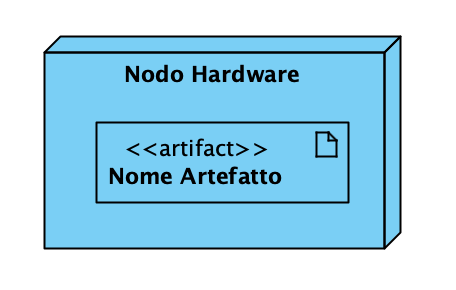
\includegraphics[scale=0.8]{img/architettura.png}
\end{figure}

\paragraph{\textcolor{cyan}{Artefatto}} L'artefatto è una copia di un'implementazione di un componente
che è stata installata su un ambiente di esecuzione. L'artefatto si dice che "\emph{manifesta}" (\verb|<<manifesta>>|) un componente.